%------------------------------------------------------------------------------
% Template file for the submission of papers to IUCr journals in LaTeX2e
% using the iucr document class
% Copyright 1999-2011 International Union of Crystallography
% Version 1.4a (17 April 2011)
%------------------------------------------------------------------------------

\documentclass[pdf]{iucr}           % DO NOT DELETE THIS LINE

     %-------------------------------------------------------------------------
     % Information about the type of paper
     %-------------------------------------------------------------------------
     \paperprodcode{a000000}      % Replace with production code if known
     \paperref{xx9999}            % Replace xx9999 with reference code if known
     \papertype{CP}               % Indicate type of article
                                  %   FA - research papers (full article)
                                  %   SC - short communications
                                  %   LA - lead article
                                  %   FE - feature articles
                                  %   ST - structural communications
                                  %   XC - crystallization communications
                                  % (Following categories rarely in LaTeX)
                                  %   AA - abstracts
                                  %   AD - addenda and errata
                                  %   BC - books received
                                  %   BR - book reviews
                                  %   CA - cif applications
                                  %   CE - current events
                                  %   CI - inorganic compounds
                                  %   CM - metal-organic compounds
                                  %   CN - cryocrystallography papers
                                  %   CO - organic compounds
                                  %   CP - computer programs
                                  %   CR - crystallographers
                                  %   CS - scientific comment
                                  %   ED - editorial
                                  %   EI - inorganic compounds
                                  %   EM - metal-organic compounds
                                  %   EO - organic compounds
                                  %   FI - inorganic compounds
                                  %   FM - metal-organic compounds
                                  %   FO - organic compounds
                                  %   IP - issue preface
                                  %   IU - iucr
                                  %   LE - letters to the editor
                                  %   LN - laboratory notes
                                  %   ME - forthcoming meetings/short courses
                                  %   MR - meeting reports
                                  %   NN - notes and news
                                  %   NP - new commercial products
                                  %   OB - obituaries
                                  %   SR - software reviews
                                  %   TE - teaching and education

     \paperlang{english}          % Can be english, french, german or russian
     %-------------------------------------------------------------------------
     % Information about journal to which submitted
     %-------------------------------------------------------------------------
     \journalcode{J}              % Indicate the journal to which submitted
                                  %   A - Acta Crystallographica Section A
                                  %   B - Acta Crystallographica Section B
                                  %   C - Acta Crystallographica Section C
                                  %   D - Acta Crystallographica Section D
                                  %   E - Acta Crystallographica Section E
                                  %   F - Acta Crystallographica Section F
                                  %   J - Journal of Applied Crystallography
                                  %   S - Journal of Synchrotron Radiation
          %--------------------------------------------------------------------
          % The following entries will be changed as required by editorial staff
          %--------------------------------------------------------------------
     \journalyr{2011}
     \journaliss{1}
     \journalvol{67}
     \journalfirstpage{000}
     \journallastpage{000}
     \journalreceived{0 XXXXXXX 0000}
     \journalaccepted{0 XXXXXXX 0000}
     \journalonline{0 XXXXXXX 0000}

%\usepackage{url, hyperref}
\usepackage{graphicx}

\begin{document}                  % DO NOT DELETE THIS LINE

     %-------------------------------------------------------------------------
     % The introductory (header) part of the paper
     %-------------------------------------------------------------------------

     % The title of the paper. Use \shorttitle to indicate an abbreviated title
     % for use in running heads (you will need to uncomment it).

\title{Dataflow: a Web-based Data Reduction Framework for Neutron Scattering}
%\shorttitle{Short Title}

     % Authors' names and addresses. Use \cauthor for the main (contact) author.
     % Use \author for all other authors. Use \aff for authors' affiliations.
     % Use lower-case letters in square brackets to link authors to their
     % affiliations; if there is only one affiliation address, remove the [a].

\cauthor[a]{William}{Ratcliff}{william.ratcliff@nist.gov}{}
\author[a]{Brian}{Maranville}
\author[a]{Paul}{Kienzle}
\author[a,b]{Andrew}{Tracer}
\author[a]{Ophir}{Lifshitz}
\author[a]{Elakian}{Kanakaraj}
\author[a]{Brendan}{Rowan}
\author[a]{Alex}{Yee}
\author[c]{Joseph}{Redmon}

\aff[a]{National Institute of Standards and Technology, Gaithersburg, Maryland  20899 \country{USA}}
\aff[b]{Princeton University, Princeton, NJ  08544 \country{USA}}
\aff[c]{Unknown}

     % Use \shortauthor to indicate an abbreviated author list for use in
     % running heads (you will need to uncomment it).

%\shortauthor{Soape, Author and Doe}

     % Use \vita if required to give biographical details (for authors of
     % invited review papers only). Uncomment it.

%\vita{Author's biography}

     % Keywords (required for Journal of Synchrotron Radiation only)
     % Use the \keyword macro for each word or phrase, e.g. 
     % \keyword{X-ray diffraction}\keyword{muscle}

%\keyword{keyword}

     % PDB and NDB reference codes for structures referenced in the article and
     % deposited with the Protein Data Bank and Nucleic Acids Database (Acta
     % Crystallographica Section D). Repeat for each separate structure e.g
     % \PDBref[dethiobiotin synthetase]{1byi} \NDBref[d(G$_4$CGC$_4$)]{ad0002}

%\PDBref[optional name]{refcode}
%\NDBref[optional name]{refcode}

\maketitle                        % DO NOT DELETE THIS LINE

\begin{synopsis}
Supply a synopsis of the paper for inclusion in the Table of Contents.
\end{synopsis}

\begin{abstract}
Neutron scattering is a technique which necessarily requires centralized facilities, 
with  distributed access (a user facility).  At such a facility, 
outside users collect data on one or more
instruments, which is typically recorded in instrument-specific coordinates.
Each user needs to do two things with this data: convert it into more universal
(physical) coordinates, and correct for any instrumentation-specific artifacts
in the data. This process is termed ``data reduction''.
A common paradigm for data reduction is for the instrument operator to create a
new program and interface for each instrument. The source
data files are reduced at user facility, where there is direct access to both
the programs and the data. The reduced output files are then carried home by the
users.
This project aims to simplify this part of the user experience. A
visual-programming interface is created in the user's browser, allowing
reduction of the source data by remote control. Reduction protocols are built up
using facility-supplied functions (in icon form) wired together to create a data
flow diagram. The user (or instrument operator) can change the reduction
protocol, and repeat the procedure as needed, and the resultant reduced files
can be downloaded by the users at will. Standard reduction protocols are made
available by the facility and instrument operator.
Changes to the protocol (and the addition of new instruments and new protocols)
will not require changes to the user interface, and instrument-specific
functions for reduction will be maintained by the instrument operators, rather
than a full-blown unique reduction program for each instrument or type of
instrument.
\end{abstract}


     %-------------------------------------------------------------------------
     % The main body of the paper
     %-------------------------------------------------------------------------
     % Now enter the text of the document in multiple \section's, \subsection's
     % and \subsubsection's as required.

\section{Introduction}

Every dataset that is produced at a neutron user facility must be reduced to physical coordinates,
with artifacts removed and uncertainties calculated, before it can be analyzed or modeled.
As a result, every type of instrument must be equipped with a software routine for performing this 
reduction.  In addition, if the reduction programs are to be distributed to users so that
they might work with the raw data at their home institutions after the experiment is complete,
each program must be compiled for multiple target platforms 
(Microsoft Windows, Mac OS, Unix, Linux, etc.) 
At a large facility this requires the writing and maintenance of dozens of programs, with multiple
target platforms for each program.
The capability for self-update (through the internet) can be built into these programs, though typically
the extra coding needed to achieve this is high.  More commonly, software updates are accomplished through
notification of all the users who might have downloaded or copied the programs, requesting that they 
download a newer version from a publicly-available repository.

We present an alternative system for providing data reduction services at a user facility: 
the Dataflow framework, consisting of
a user interface which exists solely within the user's web browser, and a centralized server which
is maintained by the facility staff.  The core functionality of the system is the graphical representation
of a reduction algorithm as a series of discrete operations on data in a user-editable workflow diagram,
an example of which can be seen in Fig. \ref{figure:sample_workflow}.

The coding required to add a new set of reduction routines
(a new instrument) to the framework is much reduced compared to writing an entirely new program
(user interface and underlying machinery) from scratch.  In addition to the workflow editing application, 
a common library for plotting data, importing files from a public (FTP) server, 
and creating and and associating files with existing reduction workflows is provided as part
of the base system.

Software updates are no longer dependent on the user, as
changes to the server are implemented without any user interaction,
and updates to the user interface code (in the browser) require only that 
the user refresh their view of the reduction site. 

Also, by presenting the user interface in a web browser, the installation requirement for users is shifted to the
browser providers.  All that is required of the user is that they run a modern browser (with Javascript
enabled.)
Current browser support is indicated in Table \ref{table:browsers}.

\section{Dataflow system}

In the client and server, every reduction session is associated with a specific, defined \emph{instrument}.
The editor for workflows allows a user to add and delete nodes in the diagram from a pool
of available modules (specific to the chosen \emph{instrument}), and attach the outputs of each node 
to the inputs of another node as necessary with wires. Each module, visually represented with 
a name and icon in the editor, corresponds to a subroutine in the 
backend, running on the server.

These modules have input and/or output terminals, which correspond to the 
inputs and/or outputs of the underlying subroutine, and wiring two terminals together in the editor
corresponds intuitively to linking those inputs and outputs in the underlying reduction chain.  In that sense 
the editor is a very simple programming environment, in which the number of available operations (modules)
is extremely limited and well-defined, as well as the number of variables (input and outputs).
Each module can also have associated configuration parameters, e.g. the desired resolution of rebinned 
data, or the magnitude of a scalar offset.  These are accessible in the editor as well, by 
clicking on the module in question on the workflow.  Parameter values are stored as part of the 
\emph{configuration} of the workflow instance when the session is saved.

The set of reduction subroutines available for an instrument typically consists
of one or more \emph{loaders} which import raw data from datafiles, and \emph{filters} which operate
on the data.  It is necessary that the \emph{loaders} and \emph{filters}
provide compatible objects within each
instrument's namespace, but it is not required that the \emph{filters} for one instrument operate on the data
of another instrument.  Thus every defined \emph{instrument} is independent of every other, and modifications
to the algorithms, data types, etc. in one will not affect any other. 

\subsection{Data management}

Sessions in the workflow editor are initiated through another online tool, the user project manager.
Users register with a unique id, and then they can log in to a personal work space.  
In this environment, the user can create new \emph{projects}, which are collections of \emph{experiments},
which are defined simply as the grouping of uploaded raw data files with a particular \emph{instrument} and
associated workflows.  

The list of associated workflows is empty when a user begins the reduction process for a new experiment,
at which point standard workflow \emph{templates} can be loaded in the editor, and then saved as specific
workflow instances associated with the \emph{experiment}.  Each reduction workflow may have more than one \emph{loader},
and so in the editor there is also a tool for associating the files in a given \emph{experiment} with individual
\emph{loaders}.  This assocation information is stored along with any user-supplied module \emph{configuration}
when the workflow instance is saved to the \emph{experiment} workspace.

\subsection{Plotting}

Data reduction is often an interactive process, in which corrections are adjusted and regions of interest
are defined midway in a reduction workflow.  Plotting of intermediate results in any workflow is possible 
by clicking on the wires themselves, triggering an evaluation of the workflow as defined up to the point of
the selected wire and plotting the result in a panel in editor window.  

Currently, plotting is supported for two types of data: 2-dimensional arrays with defined dimensions
(which are plotted as a colormap, similar to heat maps) as seen in Fig. \ref{figure:twod_plot},
and multi-dimensional data where multiple sets
of 1-d data (all of the same length) can be flexibly plotted, choosing any x- and y-axis from the sets
 (see Fig \ref{figure:nd_plot}).

\subsection{Caching}

In many reduction processes, intermediate results can be costly to calculate.  In order to
have a responsive, flexible system, small changes to the dataflow that do not require recalculation
of previous steps should not force this to happen.


\section{Implemented instruments}

The process for implementing a particular instrument, involves porting existing algorithms for data reduction 
to individual Python modules that act as filters, passing modified data to the next filter in the chain.  

Currently, three classes of instrument-specific reduction are implemented at the host institution for this 
project (NIST center for Neutron Research)

\subsection{Triple-Axis Spectrometer}

Enter Alex Yee.

\subsection{Small-Angle Neutron Scattering}

By Elakian.
For instance, in the Small-Angle Neutron Scattering (SANS) reduction, many of the algorithms used were 
adapted from exisiting Igor Pro code \cite{Kline:do5025}.

\subsection{Offspecular}

I imagine Brendan will contribute something here.


     % Appendices appear after the main body of the text. They are prefixed by
     % a single \appendix declaration, and are then structured just like the
     % body text.


\appendix
\section{Libraries used in Dataflow Application}
 
\subsection{Client}

The user interface is entirely implemented in Javascript, with added libraries as described below.
 
\subsubsection{Editor}
The main workflow (wiring) editor is implemented as a fork of the WireIt library (\emph{http://neyric.github.com/wireit/}), with added routines for running data reductions and configuring
modules with user input.
\subsubsection{Plotting}
Plotting in the client is accomplished with the jqPlot library (\emph{http://www.jqplot.com/}).
Additional plugins written as part of this project include one for handling 2-dimensional 
plotting (colormaps), as well as one for handling multi-axis data with selectors.
The jqPlot library itself depends on the jQuery library (\emph{http://jquery.com/}).
\subsubsection{Layout}
Menus and layout (exclusive of the wiring editor) were done in extJS (\emph{http://www.sencha.com/products/extjs/})
\subsection{Server}
The backend server is written in python (\emph{http://www.python.org}), 
which makes the connection between the client (web browser) and the data reduction modules, 
which are also written in Python.  

There is no particular requirement that the reduction code be written in Python, just that
the code be callable from Python.  However, because of the large available body of numerical libraries 
in Python (\emph{http://numpy.scipy.org/}), 
it was not necessary to use any other languages in the backend.
\subsubsection{Web server}
All dynamic content, including calls to run the reduction workflows and
interactive forms in the user project manager environment,
is served using the Django python library (\emph{http://www.djangoproject.com}).  
User information (project structure, sessions, experiments, uploaded data files, saved workflow instances...)
is stored in a postgresql relational database on the server, (\emph{http://www.postgresql.org/})
along with instrument definitions and default workflow templates
for each instrument type.
\subsubsection{Caching intermediate results}
As mentioned in the text, intermediate results are cached 
in memory on the server to minimize computation time and make the user interaction more responsive.  
This is  accomplished using the Redis key-value store (\emph{http://redis.io/}).  This software allows 
old entries to automatically expire after a configurable time.


\ack{Acknowledgements}

This work utilized facilities supported in part by the National Science Foundation under Agreement No. DMR-0944772.
Andrew Tracer and Joseph Redmon were supported as part of the Summer Undergraduate Research Fellowship (SURF);
Elakian Kanakaraj, Brendan Rowan and Alex Yee were supported by thed Summer High-school Internship Program (SHIP),
both of which are also part of the above grant.

The authors would like to thank Andrew Jackson, Steve Kline and Julie Borchers of the NIST Center for Neutron Research
for their invaluable assistance on this work.

%\begin{references}
%\reference{Author, A. \& Author, B. (1984). \emph{Journal} \textbf{Vol}, 
%first page--last page.}
%\end{references}
\bibliographystyle{iucr}
\bibliography{JAC_bibliography}
     %-------------------------------------------------------------------------
     % TABLES AND FIGURES SHOULD BE INSERTED AFTER THE MAIN BODY OF THE TEXT
     %-------------------------------------------------------------------------

     % Simple tables should use the tabular environment according to this
     % model

\begin{table}
\caption{Supported browsers}
\label{table:browsers}
\begin{tabular}{ l l l }      % Alignment for each cell: l=left, c=center, r=right
 Browser    &Version  &Link     \\
\hline
 Firefox      & 5.0      & \emph{http://www.firefox.com}      \\
 Chrome      & 13.0      & \emph{http://www.google.com/chrome}    \\
 Internet Explorer      & None      & Not supported      \\
\end{tabular}
\end{table}


     % Postscript figures can be included with multiple figure blocks

\begin{figure}\label{figure:sample_workflow}
\caption{Sample data reduction workflow (off-specular neutron reflectometry)}
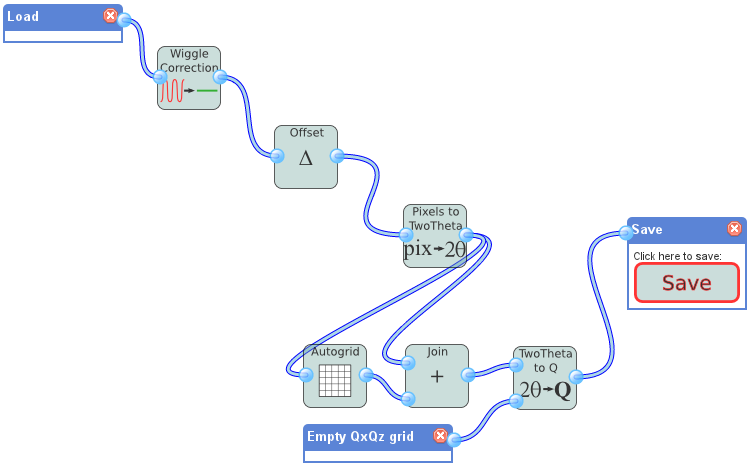
\includegraphics[width=\linewidth]{sample_diagram.png}
\end{figure}

\begin{figure}\label{figure:twod_plot}
\caption{Two-dimensional color map of data.  Log or linear mapping is selectable in
the client}
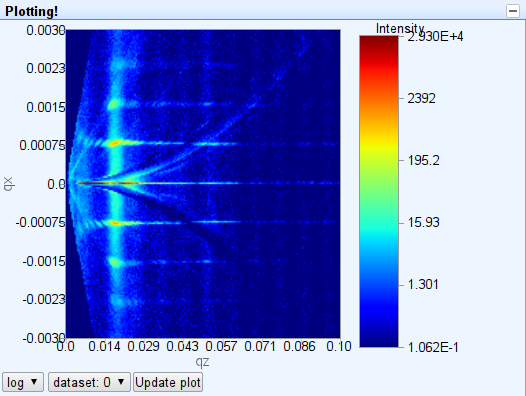
\includegraphics[width=\linewidth]{twod_plot.png}
\end{figure}

\begin{figure}\label{figure:nd_plot}
\caption{N-dimension plotter, where x- and y-axes are chosen by the user with drop-down selection inputs seen below the graph}
\includegraphics[width=\linewidth]{sample_nd.png}
\end{figure}


\end{document}                    % DO NOT DELETE THIS LINE
%%%%%%%%%%%%%%%%%%%%%%%%%%%%%%%%%%%%%%%%%%%%%%%%%%%%%%%%%%%%%%%%%%%%%%%%%%%%%%
